\section{Implement} %4.3
One of the most important idea to implement the testing environment is to modularize the function. We modularize our functions, like the AGC algorithm, the moving file script and ending file script, in a python file so we can import them as a library and call them in the main file directly. Additionally, it is necessary to remove hard coded parameters so it is easy to change the parameters like start time, end time, prepared folder address and list of generators in the main function.\\

Another noteworthy detail is we need to keep two significant digits for kp, ki and time delay. It provides an unified format that helps exporting data into analytical algorithms.\\

\begin{figure}[htbp]
\centering
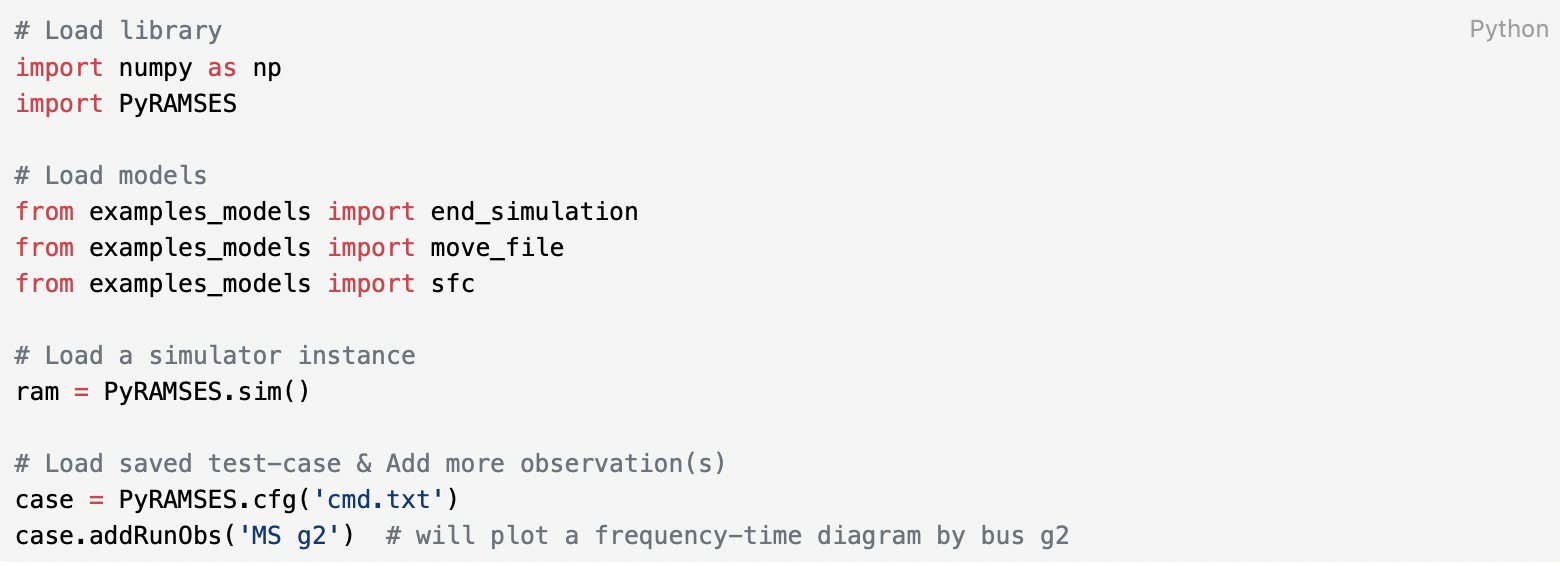
\includegraphics[width = \textwidth]{figure/4_3_code1.png}
\caption{Python: import related libraries.}
\label{4_3_code1}
\end{figure}

\begin{figure}[htbp]
\centering
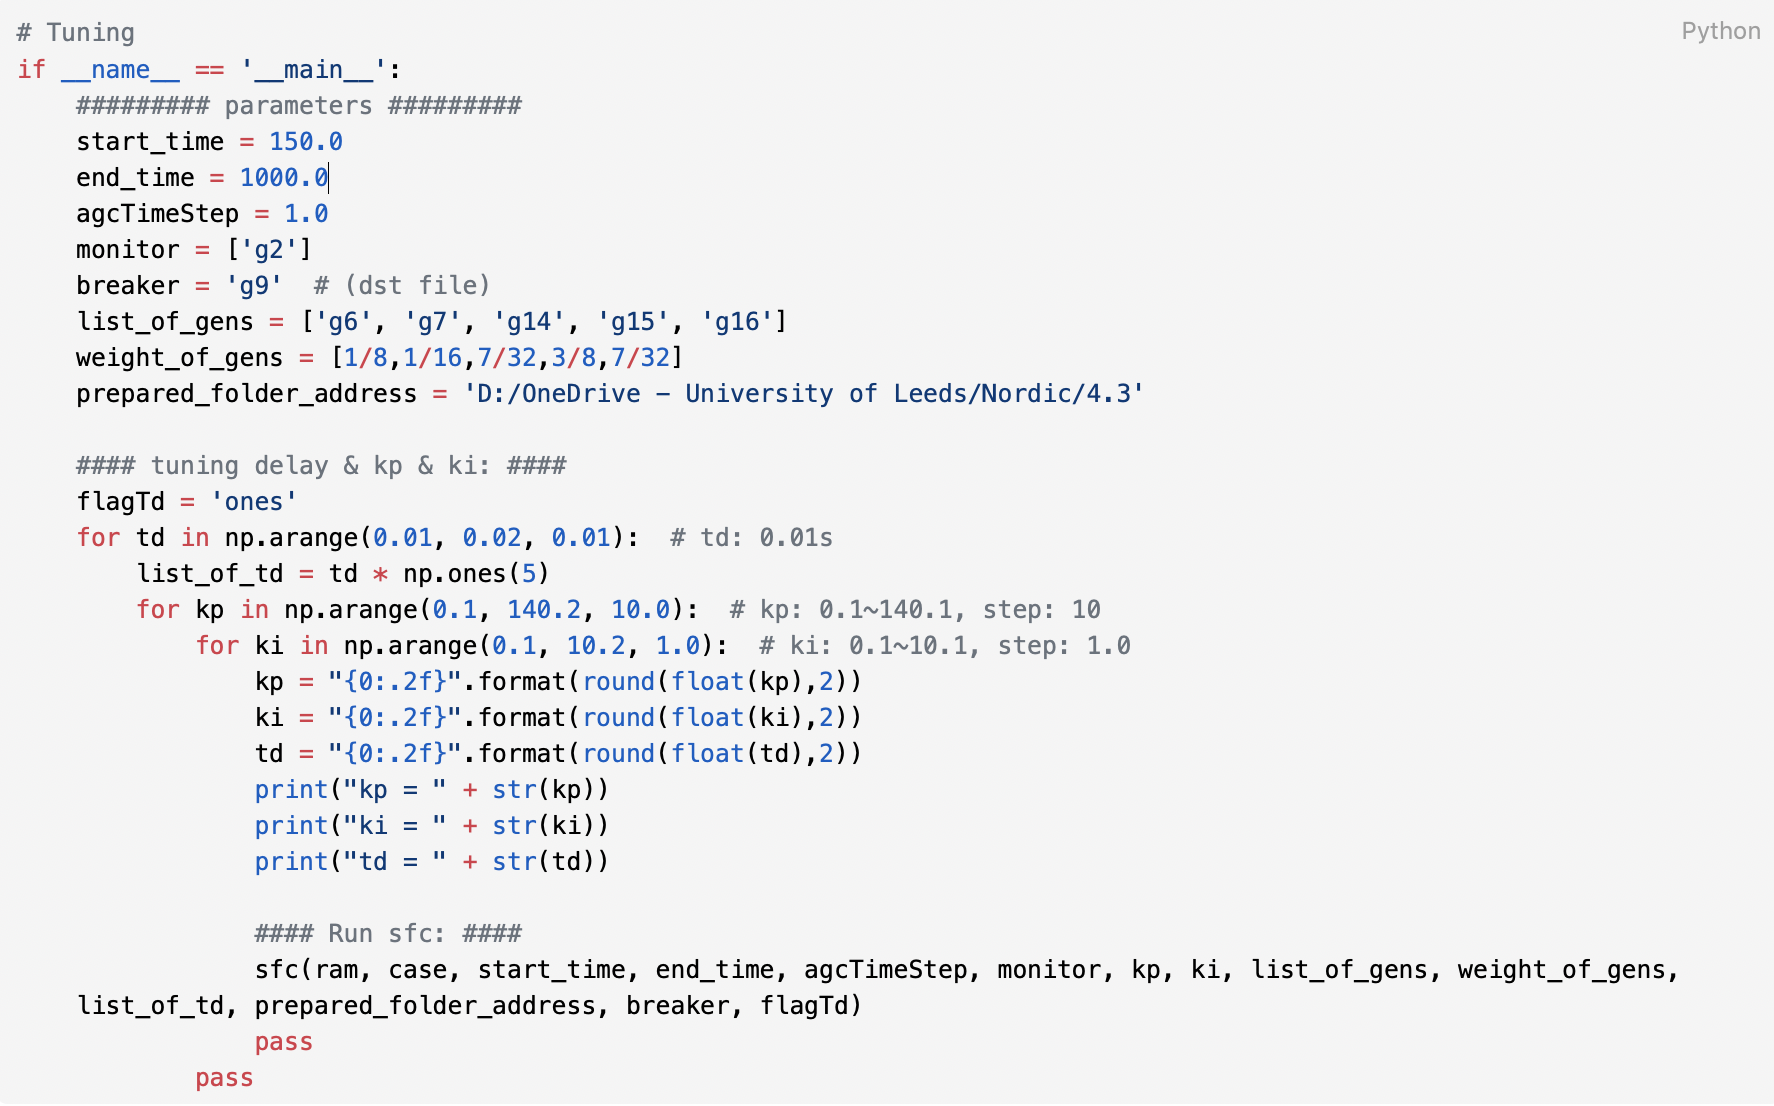
\includegraphics[width = \textwidth]{figure/4_3_code2.png}
\caption{Python: tune PI control.}
\label{4_3_code2}
\end{figure}